\documentclass[
  11pt,
  letterpaper,
   addpoints,
   answers
  ]{exam}

\usepackage{../exercise-preamble}
\usepackage{float}
\usepackage{pgfplots}
\pgfplotsset{compat=1.18}
% TikZ libraries needed for `right=.. of ..` and coordinate math
\usetikzlibrary{positioning,calc,arrows,arrows.meta}
% Alias de seguridad por si se escribe 'ikzstyle' por error
\let\ikzstyle\tikzstyle

% Comando para títulos de modo con líneas al ancho del texto
\newlength{\rulelength}
\newcommand{\modtitle}[1]{%
  \settowidth{\rulelength}{\textbf{#1}}%
  \par\addvspace{6pt}\noindent%
  \begin{tabular}{@{}l@{}}
    \rule{\rulelength}{0.5pt}\\[3pt]%
    \textbf{#1}\\[3pt]%
    \rule{\rulelength}{0.5pt}%
  \end{tabular}%
  \par\addvspace{8pt}%
}

\begin{document}

% Configuración del encabezado usando comandos de la clase exam
\pagestyle{headandfoot}
\extraheadheight{0.5in}
\firstpageheader{\textit{Microondas}}{}{EL7029}
\runningheader{\textit{Microondas}}{}{EL7029}
\firstpagefooter{}{\thepage}{}
\runningfooter{}{\thepage}{}
\headrule

% Numeración de página
\pagenumbering{arabic}

% Portada
\begin{center}
    \vspace*{1cm}
    
    % Logo superior
    
\includegraphics[width=0.5\textwidth]{../fcfm_die}
    
    \vspace{2cm}
    
    % Líneas decorativas superiores
    
\begin{tikzpicture}
        \draw[line width=2pt, black!70] (0,0) -- (10,0);
        \draw[line width=0.5pt, black!50] (0,0.2) -- (10,0.2);
    \end{tikzpicture}
    
    \vspace{1cm}
    
    % Título principal
    {\fontsize{28}{34}\selectfont\bfseries 
   Microondas}
    
    \vspace{0.5cm}
    
    {\Large\textbf{EL7029}}
    
    \vspace{0.3cm}
    
    {\large Lineas de Transmisión y Carta Smith}
    
    \vspace{1cm}
    
    % Líneas decorativas inferiores
    
\begin{tikzpicture}
        \draw[line width=0.5pt, black!50] (0,0) -- (10,0);
        \draw[line width=2pt, black!70] (0,0.2) -- (10,0.2);
    \end{tikzpicture}
    
    \vspace{1.5cm}
    
    % Subtítulo
    {\LARGE\itshape Auxiliar 1}
    
    \vspace{1cm}

    % Cuadro semestre y profesores
    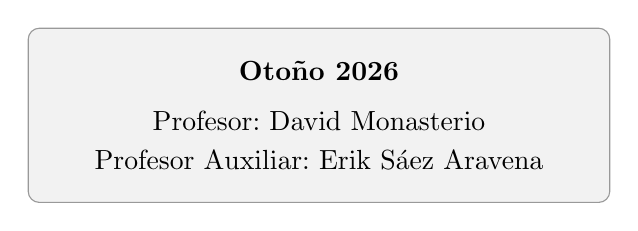
\begin{tikzpicture}
        \node[draw=black!40, fill=black!5, rounded corners=4pt,
              inner xsep=24pt, inner ysep=12pt, align=center] {
            \textbf{Otoño 2026}\\[6pt]
            Profesor:\ David Monasterio\\[2pt]
            Profesor Auxiliar:\ Erik Sáez Aravena
        };
    \end{tikzpicture}

    \vfill

    \vspace{1cm}
    
\end{center}

\newpage

\begin{questions}
  \question a
\end{questions}
\end{document}